\ylDisplay{Nõguspeegel} % Ülesande nimi
{Tundmatu autor} % Autor
{lõppvoor} % Voor
{2006} % Aasta
{G 2} % Ülesande nr.
{3} % Raskustase
{
% Teema: Geomeetriline-optika
\ifStatement
On teada esemelt lähtunud ühe kiire suund enne ja pärast peegeldumist sfääriliselt nõguspeeglilt. Teades eseme $AB$ ja optilise peatelje asukohta, konstrueerige eseme kujutis ja tähistage nõguspeegli fookuse asukoht.

\begin{center}
	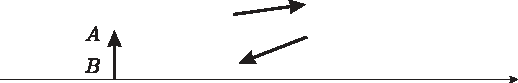
\includegraphics[width=0.9\linewidth]{2006-v3g-02-yl}
\end{center}
\fi


\ifHint
Nõguspeegli pinnalt peegeldunud kiirte nurgapoolitajad läbivad peegli kõverusraadiuse keskpunkti.
\fi


\ifSolution
Jooniselt antud kiire kahe osa pikenduste lõikepunkt vastab nõguspeegli pinnale ning kiirte nurgapoolitaja ja optilise peatelje lõikepunkt annab nõguspeegli kõverusraadiuse keskpunkti $O$. Fookuse leidmiseks paneme tähele, et nõguspeegli fookuskaugus on pool kõverusraadiusest, kus kõverusraadiuse saame mõõta jooniselt. Edasi saame fookuse kaudu konstrueerida teise punktist $A$ alguse saanud kiire käigu ning määrata eseme kujutise asukoha.

\begin{center}
	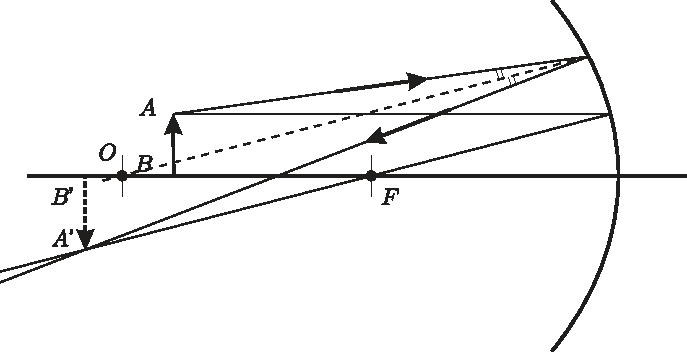
\includegraphics[width=\linewidth]{2006-v3g-02-lah}
\end{center}
\fi
}